\section{Client Unit}
\label{sec:client}


\emph{Client} unit is output type unit that connects to BGPmon. \emph{Client} unit receives stream of XML  update messages from BGPmon and prints it in human readable view. The output from \emph{Client} unit includes important debugging values like network prefix and AS path.  \emph{Client} does not rely on source of input to BGPmon, it uses XML messages from BGPmon. Overall, \emph{Client} unit is designed to achieve following goals:

\begin{itemize}
\item{BGPmon provide XML messages in output: its important to verify that BGPmon sends XML update messages to the \emph{Client} unit.}
\item{XML messages include values that were configured by user of framework at \emph{Peer}, \emph{MRT} or \emph{Chain} units.}
\end{itemize}


\subsection{IPv4 Client Unit}

\begin{figure}
\centering
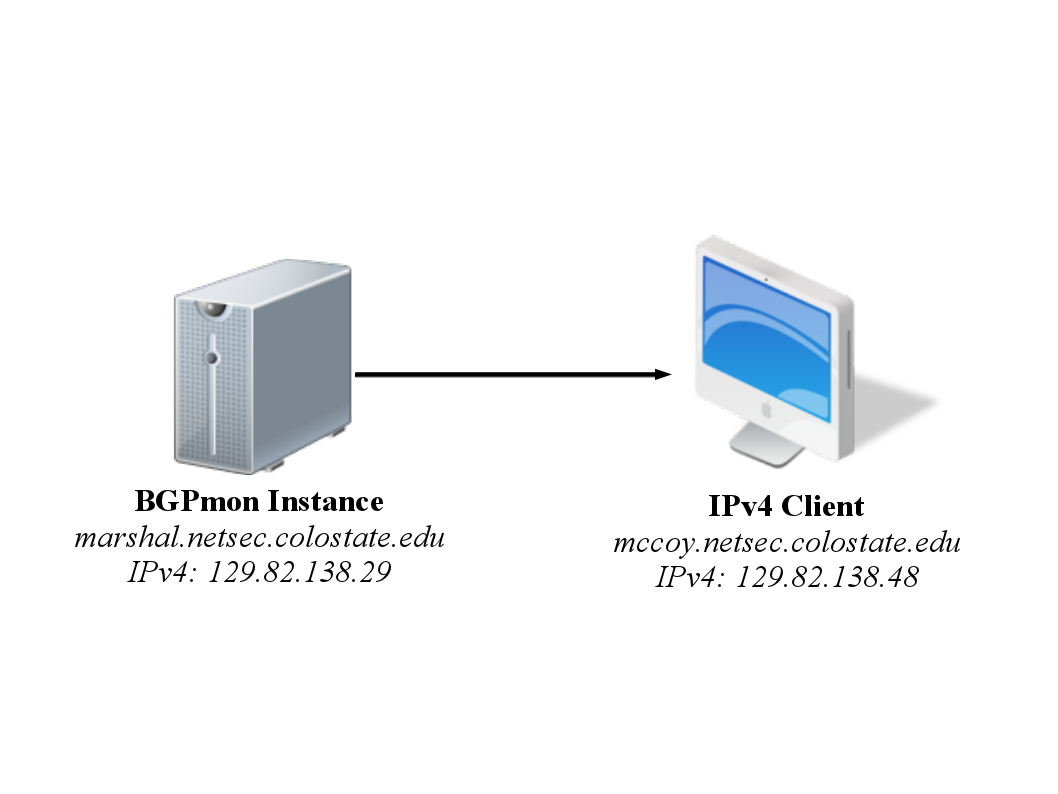
\includegraphics[scale=0.30]{figs/ipv4-client.png}
\caption{An overview of IPv4 Client Unit.}
\label{clientfig}
\end{figure}

Figure \ref{clientfig} shows unit design: it has \emph{IPv4 Client} unit and BGPmon test instance. \emph{IPv4 Client} unit is installed on \emph{mccoy.netsec.colostate.edu} with \emph{129.82.138.48} IPv4 address.  BGPmon test instance is configured on \emph{marshal.netsec.colostate.edu} with \emph{129.82.138.29} IP address. 


\subsubsection{IPv4 Client Unit Configuration}

\emph{IPv4 Client} unit is application that connects to BGPmon test instance and receives XML update messages.    \emph{IPv4 Client} supports following input values:

\begin{verbatim}
$ statclient [IP] [PORT]
\end{verbatim}

where \emph{[IP]} is IP address of BGPmon instance. \emph{[PORT]} is a port of BGPmon server.


\subsubsection{BGPmon Test Unit Configuration}

To enable  XML feed on BGPmon instance, user has to be logged to \emph{marshal.netsec.colostate.edu} and ensure that BGPmon process is up and running.  To enable stream of XML messages, run   run following command in \emph{configuration mode} in  CLI:

\begin{verbatim}
marshal(config)#client-listener enable
\end{verbatim}

BGPmon test instance starts  to listen TCP connections on \emph{50001} and \emph{50002} on \emph{marshal.netsec.colostate.edu}. Port \emph{50001} provides a stream of XML update messages, port \emph{50002} sends XML table messages.

\subsubsection{Result reporting}

\emph{Client} unit prints BGP messages in human readable format. This output can be used in debugging any of three types of input to BGPmon.  For instance, user may configure setup of BGP peer that announce \emph{11.0.0.0/8} network prefix. After BGP peer establish BGP peering session with BGPmon, it will send BGP update message to BGPmon. \emph{Client} will receive XML update message and print network information to the user. 